\documentclass[11pt]{report}
\usepackage[abgabe]{protokoll}
\lstset{literate=
  {á}{{\'a}}1 {é}{{\'e}}1 {í}{{\'i}}1 {ó}{{\'o}}1 {ú}{{\'u}}1
  {Á}{{\'A}}1 {É}{{\'E}}1 {Í}{{\'I}}1 {Ó}{{\'O}}1 {Ú}{{\'U}}1
  {à}{{\`a}}1 {è}{{\`e}}1 {ì}{{\`i}}1 {ò}{{\`o}}1 {ù}{{\`u}}1
  {À}{{\`A}}1 {È}{{\'E}}1 {Ì}{{\`I}}1 {Ò}{{\`O}}1 {Ù}{{\`U}}1
  {ä}{{\"a}}1 {ë}{{\"e}}1 {ï}{{\"i}}1 {ö}{{\"o}}1 {ü}{{\"u}}1
  {Ä}{{\"A}}1 {Ë}{{\"E}}1 {Ï}{{\"I}}1 {Ö}{{\"O}}1 {Ü}{{\"U}}1
  {â}{{\^a}}1 {ê}{{\^e}}1 {î}{{\^i}}1 {ô}{{\^o}}1 {û}{{\^u}}1
  {Â}{{\^A}}1 {Ê}{{\^E}}1 {Î}{{\^I}}1 {Ô}{{\^O}}1 {Û}{{\^U}}1
  {œ}{{\oe}}1 {Œ}{{\OE}}1 {æ}{{\ae}}1 {Æ}{{\AE}}1 {ß}{{\ss}}1
  {ű}{{\H{u}}}1 {Ű}{{\H{U}}}1 {ő}{{\H{o}}}1 {Ő}{{\H{O}}}1  
  {ç}{{\c c}}1 {Ç}{{\c C}}1 {ø}{{\o}}1 {å}{{\r a}}1 {Å}{{\r A}}1
  {€}{{\EUR}}1 {£}{{\pounds}}1
}
\graphicspath{
  {pictures/}
}
\lstset{inputpath=source/}
\version{0.1$\alpha$}
\datum{\today}

%%
%% Titel, Autor und Betreuer
%%
\fachbereich{VII -- Hallo - Mechatronik - Optometrie --} 
\studiengang{Elektrotechnik - Schwerpunkt Elektronische Systeme}
\autor{Robby Kozok, Nic Frank Siebenborn, Pascal Kahlert}
\titel{Realisierung und Analyse des FIR-Filters} 
\untertitel{Laborbericht}
\modul{Digitale Signalverarbeitung III}
\betreuerFeld{
  \begin{tabular}{lr}
    \multicolumn{2}{l}{\textbf{Lehrkraft}}\\
    Prof.~Dr.-Ing~Marcus~Purat & Beuth Hochschule für Technik\\
  \end{tabular}
}
%%
%% Abkürzungen
%%
\makenoidxglossaries

\newacronym{fda}{FDA}{Filter Design and Analysis}





\begin{document}

\pagestyle{fancy}

%% Titelseite
\maketitle
\clearpage

%% Leerseite
\newpage

%\chapter*{Einleitung}

%% Einfügen des genutzten Aufgabenblattes. 
\clearpage
%% Seitenzahlen
\pagenumbering{roman}

%% Inhaltsverzeichnis
\tableofcontents

%% Abbildungsverzeichnis


%%Titelseite


\pagenumbering{arabic}


%%Kapitel
\chapter{Realisierung des FIR-Filters}\label{Cha:RealFIR}
\section{Aufgabenstellung}
Die Aufgabenstellung bestand darin, ein FIR - Mittelwertfilter zu realisieren und auf verschieden Weisen zu implementieren.
Anschließend wurden die Implementierungen auf ihre Leistung untersucht und verglichen. Es handelt sich jedes mal um ein FIR - Mittelwertfilter vierter Ordnung.

\section{Durchf\"uhrung}
Gemäss des Umdrucks wurde ein Projekt erstellt und die entsprechenden Dateien angefügt. In einem ersten Teil wurde dann die Sprungantwort mithilfe einer Simulation durch händisches verändern der Eingangswerte ermittelt und aufgenommen. 
In der folgenden Tabelle sind die von uns manipulierten Werte und die in sDAC1L resultierenden Werte aufgezeigt.
\begin{center}
\begin{tabular}{|c|c|}
\hline 
Eingang & Ausgang \\ 
\hline 
0 & 0 \\ 
\hline 
25716 & 5143 \\ 
\hline 
25716 & 10286 \\ 
\hline 
25716 & 15429 \\ 
\hline 
25716 & 20572 \\ 
\hline 
25716 & 25716 \\ 
\hline 
25716 & 25716 \\ 
\hline 
%%\caption{Erfassung der Sprungantwort\textunderscore Mode}
\end{tabular} 
\end{center}

Im nachfolgenden Bild ist diese Annäherung grafisch dargestellt. Man erkennt gut, dass sich der Ausgangswert sukzessive und linear dem Eingangswert annähert. 
Dies passiert in fünf Schritten, wie es für ein solches Filter üblich ist und entspricht damit den Erwartungen
\begin{figure}[H]
  \centering
    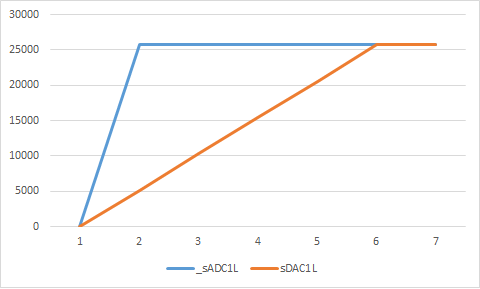
\includegraphics[width=\textwidth]{Sprungantwort1.png}
  \caption{Sprungantwort des FIR Filters\textunderscore Mode\textunderscore Sprungantwort1.png}
  \label{fig:SprAW1.png}%%Konvention figures immer mit fig:
\end{figure}
 %%%%%%%%%%%%%%%%%%%%%%%%vergleich mit vorbereitung
 In der Vorbereitung wurde die Sprungantwort eines Filters vierter Ordnung ermittelt, welche auf dem folgenden Bild zu sehen ist.
 %%%%%%%%%%bild SprungantwortMittelwert.png
 \begin{figure}[H]
  \centering
    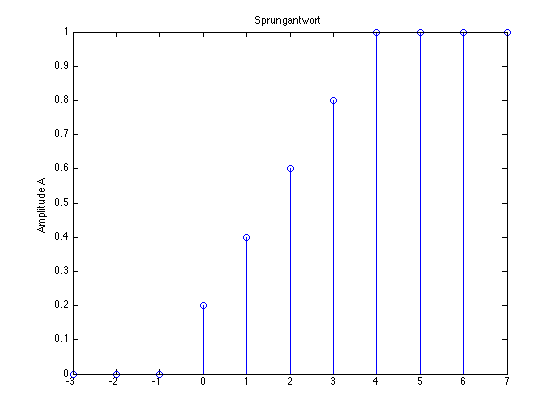
\includegraphics[width=\textwidth]{SprungantwortMittelwert.png}
  \caption{Sprungantwort des FIR Filters aus der Vorbereitung\textunderscore Mode\textunderscore SprungantwortMittelwert.png}
  \label{fig:SprAW.png}%%Konvention figures immer mit fig:
\end{figure}
 Trotz der Unterschiedlichen Darstellungsarten ist eindeutig zu sehen, dass sich die Filter gleich verhalten.
 
 Es wurde eine Programmzyklenzahl von 1672 ermittelt.
 
 Im nächsten Schritt wird diese Herangehensweise wiederholt, diesmal allerdings mit Zahlen im 1.15 Format. Dazu wurden die Variablen auf den Typ short Integer im C-Code angepasst.\\
 \begin{adjustbox}{width=\textwidth,height=\textheight,keepaspectratio}
 \begin{lstlisting}[title=fir.c]{fir.c}
#include "fir.h"

short fir(short sInput, FIRstate *pFIR) {

	int k;
//	float acc; //Datentyp gemaess Aufgabe angepasst
	int acc;
	
	*(pFIR->p++)=sInput;	// store current sample in delayline
	if ( pFIR->p >= pFIR->d + pFIR->N) pFIR->p-=pFIR->N;

	for (acc=0,k=0;k<pFIR->N;k++) {
		acc += (*(pFIR->p++) * pFIR->h[k]);
		if ( pFIR->p >= pFIR->d + pFIR->N) pFIR->p-=pFIR->N;
	}
	
	return (short)(acc >> 15); //rightshift um nur hoeherwertige Bits zu verwenden
}
\end{lstlisting}
\end{adjustbox}
Wie zu sehen ist wurden im Vergleich zur Ursprungsversion zwei Änderungen vorgenommen: acc wurde zu einem Integer und der Typecast im return-statement wurde um einen Rechtsshift erweitert. Die erste \"Anderung erklärt sich aus der Aufgabe da mit short Integer gerechnet werden sollte, wobei acc das ergebnis einer Multiplikation ist, welche so viele Bits hat wie beide Summanden zusammen, deshalb int statt short. Der Rechtsshift sorgt daf\"ur, dass nur die 15 h\"oherwertigen Bits zum short getypecastet werden.\\\par
Wir \"uberprüften die Funktionsweise wie oben und erhalten folgende 
Messwerte:\\
\begin{center}
\begin{tabular}{|c|c|}
\hline 
0 & 0 \\ 
\hline 
0,5 & 0,1 \\ 
\hline 
0,5 & 0,2 \\ 
\hline 
0,5 & 0,3 \\ 
\hline 
0,5 & 0,4 \\ 
\hline 
0,5 & 0,5 \\ 
\hline 
0,5 & 0,5 \\ 
\hline 
\end{tabular} 
\end{center}
woraus folgende Grafik entsteht.
\begin{figure}[H]
  \centering
    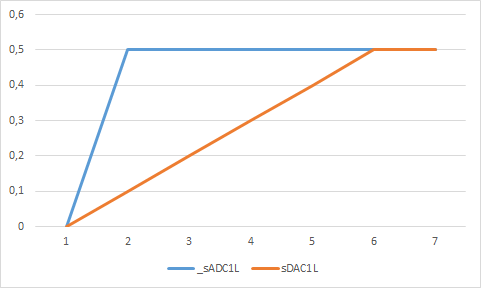
\includegraphics[width=\textwidth]{Sprungantwort2.png}
  \caption{Sprungantwort des FIR Filters im short Integer Format\textunderscore Mode\textunderscore Sprungantwort2.png}
  \label{fig:SprAW2.png}%%Konvention figures immer mit fig:
\end{figure}
Wieder sind alle Werte wie erwartet.
Die Messung ergab eine Programmzyklenzahl von 764, was eine deutliche Leistungsverbesserung gegen\"uber des Versuches zuvor ist, was sich darin begr\"undet, dass der DSP f\"ur 16-Bit-Operationen optimiert ist.\\
In einem weiteren Optimierungsschritt wird das Filter nun in Assembler umgesetzt um Optimierungen zu nutzen die der Compiler sonst nicht nutzt, wir erwarten eine schnellere Abarbeitung.
Dazu wurde die Datei fir.asm im Bereich f\"ur die Funktion \textunderscore fir: angepasst:
\begin{adjustbox}{width=\textwidth,height=\textheight,keepaspectratio}
 \begin{lstlisting}[title=fir.c]{fir.c}
//!! Begin of Setting I, L, and B regs	
B1 = P1; //Basis: Erstes Verzoegerungsglied, hier delay line.
R1 = R1 << 1; //Mal 2, weil Short Int 2 Byte hat.
L1 = R1; // Laenge festlegen auf 2 mal 2 Byte.
I1 = P2; // I1 auf Read/Write legen
I2 = P0; // I2 auf Filterkoeffizienten
//!! End of Setting I, L, and B regs

\end{lstlisting}
\end{adjustbox}
Die Register werden so konfiguriert, dass die Funktionalität des Filters abgebildet wird, vergleiche hierzu den kompletten Code siehe Anhang. I2 beinhaltet dabei die \"ubergebenen Filterkoeffizienten und wird mit I1 multipliziert, was den aktuell \"ubergebenen Werten entspricht. L1 ist die L\"ange des zyklischen Speichers und muss damit der Ordnung des Filters multipliziert mit dem Speicherbedarf eines Wertes, hier 2 Byte multipliziert werden. Der Anfang des Speichers muss logischer Weise der Anfang des Filters sein, hier Parameter P1.\\

Auf die Aufnahme einer Messreihe und der entsprechenden Grafik wird der Übersichtlichkeit halber ab hier verzichtet, da die Versuche gezeigt haben, dass die Messreihen jedes mal identisch aussehen, lediglich die Programmzyklenzahl hat sich verändert. Sie beträgt in diesem Fall 100, was einer weiteren Performanceverbesserung und unseren Erwartungen aus oben gegebenem Grund entspricht.\\
Der letzte Optimierungsschritt nutzt die Fähigkeit des DSPs zur parallelen Abarbeitung zweier MAC-Operationen aus. Dazu wurde die Funktion zum Aufruf der Filterfunktionalität wie in der Aufgabe beschrieben ersetzt, die isr.c zum Aufruf der Stereofunktion durch Auskommentieren verändert und fir.asm wie folgt angepasst. Im Teil \textunderscore fir\textunderscore stereo: wurden Register wie folgt angepasst.

\begin{adjustbox}{width=\textwidth,height=\textheight,keepaspectratio}
 \begin{lstlisting}[title=fir.c]{fir.c}
//!! Begin of Setting I, L, and B regs	
B1 = P1; //Basis: Erstes Verzoegerungsglied, hier delay line.
R1 = R1 << 2; // 4*R1 da 32 Bit -> 8Bit*4=32
L1 = R1; // Laenge festlegen auf 4 mal 2 Byte.
I1 = P2; // I1 auf Read/Write legen
I2 = P0; // I2 auf Filterkoeffizienten
//!! End of Setting I, L, and B regs
\end{lstlisting}
\end{adjustbox}
Diese Konfiguration entspricht der selben wie in der Aufgabe zuvor, mit dem Unterschied, dass der Speicher doppelt so lang ist. Dies begr\"undet sich darin, dass nun zwei Werte gleichzeitig bearbeitet werden.\\
Auch in diesem Fall wurde die Programmlaufzeit ermittelt und ist mit 52 Zyklen die schnellste, auch dies haben wir auf Grund der nun parallelen Abarbeitung erwartet.



\section{Auswertung}
Es soll die maximal m\"ogliche Anzahl an Ausf\"uhrungszyklen für die Laborsituation anhand der ermittelten Programmzyklenzahlen berechnet werden.\\
\begin{center}
\begin{tabular}{|c|c|}
\hline 
Art der Realisierung & Anzahl Programmzyklen \\ 
\hline 
Fliesskommarealisierung in C & 1672 \\ 
\hline 
Festkommarealisierung in C & 764 \\ 
\hline 
Festkommarealisierung in asm & 100 \\ 
\hline 
Festkommarealisierung in asm mit SIMD & 52 \\ 
\hline 
\end{tabular} 
\end{center}

Bei einer Abtastfrequenz von \( f_{abtast}=48kHz \) und einer Befehlsfrequenz von \( f_{Befehl}=500MHz \) ergibt sich eine maximale Programmzyklenzahl von
\begin{equation}
N_{ZyklMax} \leq f_{Befehl}/f_{abtast} \leq 10416 
\end{equation}
Zur Berechnung der maximalen Filterordnung in den zwei F\"allen der C-Implementierung gen\"ugt ein einfacher Dreisatz:
\begin{equation}
N_{OrdnMaxCFloat} + 1 \leq 5*10416/1672\leq 31,15 \text{ ergibt }  N_{OrdnMaxCFloat}=30
\end{equation}
\begin{equation}
N_{OrdnMaxC1.15} + 1 \leq 5*10416/764\leq 68,17 \text{ ergibt }  N_{OrdnMaxC1.15}=67
\end{equation}
Bei den Realisierungen in Assembler ist der Overhead hingegen zu beachten, da die Schleifenabarbeitung genau einen Befehlstakt betr\"agt. Daher wird von der genutzten Zyklenzahl zwei mal die Filterkoeffizientenzahl abgezogen(zwei, da der linke und der rechte Audiokanal berechnet werden m\"ussen). Und das Ergebnis dann halbiert, wegen der nicht parallelen Berechnung.
\begin{equation}
N_{OrdnMaxAsm} + 1 \leq (10416-(100-2*5)/2)\leq 5163 \text{ ergibt }  N_{OrdnMaxAsm}=5162
\end{equation}
Bei der Berechnung dieser Werte mit SIMD-Befehlen f\"allt der Faktor 2 nat\"urlich weg.
\begin{equation}
N_{OrdnMaxAsmSIMD} + 1 \leq 10416-(52-5)\leq 10369 \text{ ergibt }  N_{OrdnMaxAsmSIMD}=10368
\end{equation}
Die Berechnungen st\"utzen die Erwartung, dass die Programme immer performanter wurden und dadurch auch h\"oherwertige Filter verarbeiten k\"onnen.
\chapter{Analyse des FIR-Filters}
\section{Aufgabenstellung}
Im zweiten Teil des Laborversuchs sollte das Verhalten des Filters mit den 
Ergebnissen der Vorbereitung verglichen werden.\\ Außerdem soll ein FIR-Filter 
h\"oherer Ordnung, mithilfe eines MatLab-Tools entworfen werden.
\section{Durchf\"uhrung}
Zur Analyse des in \ref{Cha:RealFIR} erstellten Filters wurde ein Sinussignal 
an den Eingang des Filters angelegt werden. Durch alternieren der Frequenzen des 
Signals, konnten wir dann die Nullstellen anhand der Amplitude des 
Ausgangssignals ermitteln.\\
Diese Analyse wurde dann mit Aufnahme des Amplitudenganges vertieft.\\
Zum aufnehmen der Sprungantwort wurde dann ein Rechtecksignal mit 2000Hz.
Diese Frequenz wurde ausgewählt, da ein zu schnelles Signal dazu führen würden, dass 
die Sprungantwort des Filters nicht in eine komplette Periode des Rechtecksignals passen 
w\"urde.\\\par
Im zweiten Teil dieses Versuchteils, wurde ein Filter h\"oherer Ordnung mit 
einem \gls{fda}-Tool entworfen. Dabei sollte folgende Parameter genutzt werden:
\begin{itemize} 
\item Equiripple-Charakteristik
\item Passband-Frequenz: 3400 Hz
\item Stoppband-Frequenz: 4000 Hz 
\item Abtastfrequenz: 48000 Hz 
\item Passband-Welligkeit: 2dB 
\item Stoppband-D\"ampfung: 80dB
\end{itemize}
\newpage
Die dadurch erzeugten Filter Koeffizienten wurden dann im fractional Format in 
die bereits vorhandene C-Header-Datei eingefügt. Dies ist in dem untenstehenden Quellcode-Ausschnitt zu sehen.\\
\begin{adjustbox}{width=\textwidth, keepaspectratio} 
  \label{code:procdataKompFIR}
  \begin{lstlisting}[title=process\textunderscore data\textunderscore KompFIR.c]
// Definition der Filterkoeffizienten
#define N_FILT 184 // Anzahl der Koeffizienten

const short coef[N_FILT] = {
       -5,    -12,    -25,    -43,    -67,    -98,   -132,   -168,   -200,
     -226,   -239,   -237,   -215,   -175,   -119,    -51,     21,     89,
      144,    179,    189,    173,    134,     79,     18,    -39,    -81,
     -100,    -92,    -59,     -7,     54,    112,    155,    174,    163,
      124,     64,     -5,    -69,   -115,   -132,   -114,    -64,      9,
       91,    164,    213,    224,    193,    124,     31,    -70,   -155,
     -206,   -209,   -160,    -66,     56,    181,    282,    334,    323,
      245,    112,    -52,   -214,   -336,   -390,   -355,   -231,    -36,
      196,    416,    575,    630,    555,    347,     33,   -336,   -686,
     -939,  -1017,   -864,   -454,    204,   1058,   2024,   2996,   3856,
     4500,   4843,   4843,   4500,   3856,   2996,   2024,   1058,    204,
     -454,   -864,  -1017,   -939,   -686,   -336,     33,    347,    555,
      630,    575,    416,    196,    -36,   -231,   -355,   -390,   -336,
     -214,    -52,    112,    245,    323,    334,    282,    181,     56,
      -66,   -160,   -209,   -206,   -155,    -70,     31,    124,    193,
      224,    213,    164,     91,      9,    -64,   -114,   -132,   -115,
      -69,     -5,     64,    124,    163,    174,    155,    112,     54,
       -7,    -59,    -92,   -100,    -81,    -39,     18,     79,    134,
      173,    189,    179,    144,     89,     21,    -51,   -119,   -175,
     -215,   -237,   -239,   -226,   -200,   -168,   -132,    -98,    -67,
      -43,    -25,    -12,     -5
};// Von MatLab generierte Filter Koeffizienten
  \end{lstlisting}
\end{adjustbox}

In Zeile 2 wurde die Anzahl der Koeffizienten festgelegt und in Zeile 4 bis Zeile 
26 wurden die Koeffizienten eingetragen, außer diesen \"Anderungen war es nicht 
notwendig den Quellcode anzupassen.\newpage


\section{Auswertung des Mittelwert FIR-Filter}
F\"ur diesen Aufgabenteil haben wir jeweils zwei 
Minimalf\"alle und zwei normale F\"alle ausgew\"ahlt, alle Eingangssignale haben eine Amplitude von 1V. Diese sind in Abbildung 
\ref{fig:5k1V} bis Abbildung \ref{fig:19k21V} 
\begin{figure}[H]
  \centering
    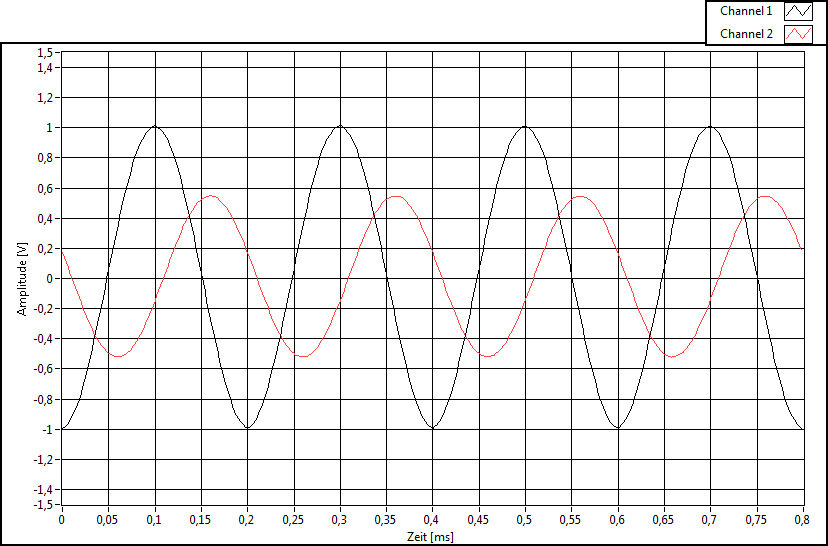
\includegraphics[width=\textwidth]{fir5k1VMax.png}
  \caption{Frequenz: 5 kHz}
  \label{fig:5k1V}
\end{figure}
In Abbildung \ref{fig:9k61V} und Abbildung \ref{fig:19k21V} sind die 
Auswirkungen der Nullstellen 
des Filters zu sehen. Dort ist das Ausgangssignal fast Null. In Abbildung \ref{fig:5k1V} 
und Abbildung \ref{fig:15k1V} ist zu sehen, dass das Signal ged\"ampft ist aber 
deutlich gr\"oßer Null ist.
Diese Ergebnisse entsprechen der Vorbereitung. \\\par
Die Verz\"ogerung zwischen Eingangssignal und Ausgangssignal ist, wie bereits im 
ersten Laborversuch, dem Versuchsaufbau zu verschulden, allerdings treten nun 
durch den Filter wiederum Verz\"ogerungen auf.
Diese Verz\"ogerungen sind damit zu erkl\"aren, dass der FIR Filter den Ausgang 
immer aus den letzten N\textunderscore FILT Werten bestimmt. Damit folgt auch das 
ausgegebene Signal diesem Muster.
\begin{figure}[H]
  \centering
    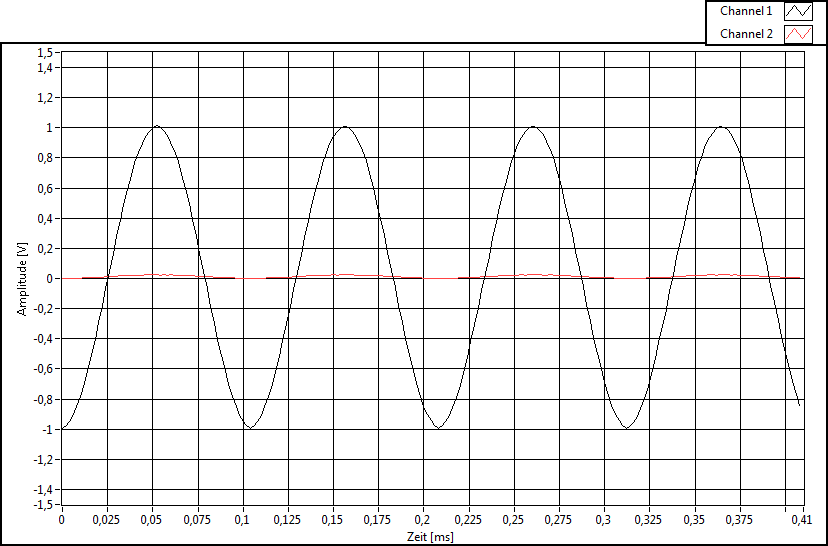
\includegraphics[width=\textwidth]{fir9k61VMin.png}
  \caption{Frequenz: 9,6 kHz}
  \label{fig:9k61V}
\end{figure}
\begin{figure}[H]
  \centering
    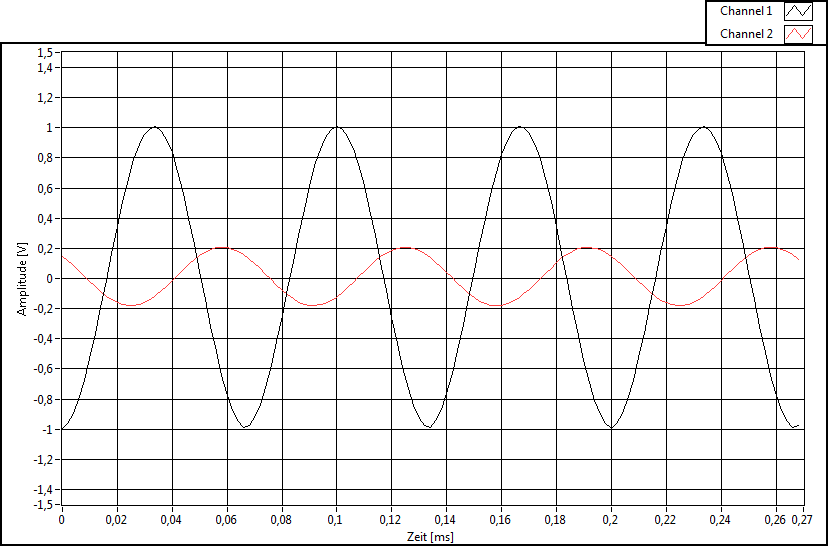
\includegraphics[width=\textwidth]{fir15k1VMax.png}
  \caption{Frequenz: 15 kHz}
  \label{fig:15k1V}
\end{figure}
\begin{figure}[H]
  \centering
    \includegraphics[width=\textwidth]{fir19k21VMin.png}
  \caption{Frequenz: 19,2 kHz}
  \label{fig:19k21V}
\end{figure}\newpage
Die Nullstellen lassen sich des weiteren im Amplitudengang ablesen, dieser ist 
in \ref{fig:AmpgangFIRMit} zu sehen. Dort ist bei ungefähr 9,6 kHz ein Einbruch 
auf -68dB und ein Einbruch auf -65dB bei 19,2 kHz zu sehen.\\
Auff\"allig, aber nicht weiter \"uberraschend, ist der Verlauf des Signals bei ca. 24 kHz. 
Dieser folgt aus dem Tiefpassverhalten des Codecs.
\begin{figure}[H]
  \centering
    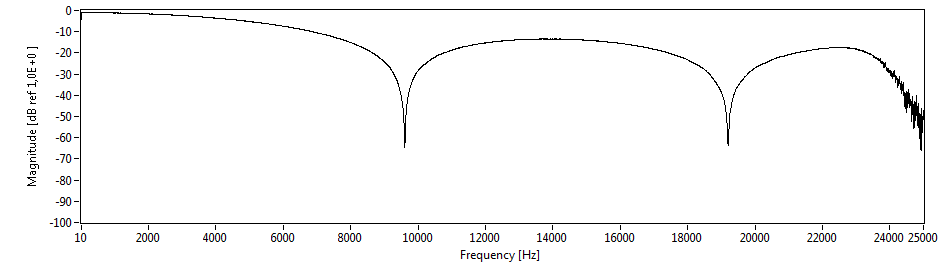
\includegraphics[width=\textwidth]{freqgang22_1.png}
  \caption{Amplitudengang des FIR Mittelwertfilters}
  \label{fig:AmpgangFIRMit}
\end{figure}
Im weiteren Verlauf soll nun die Sprungantwort des Filters analysiert werden.
\begin{figure}[H]
  \centering
    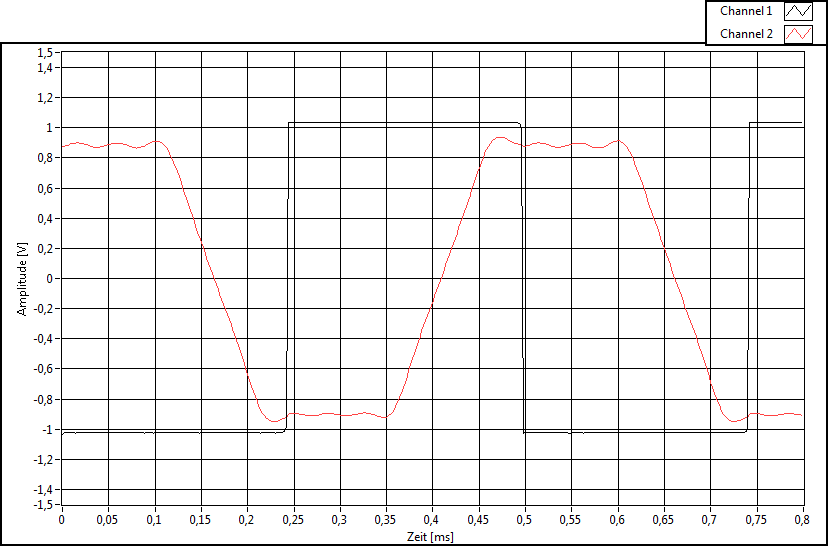
\includegraphics[width=\textwidth]{sq2k1v.png}
  \caption{Sprungantwort des FIR Mittelwertfilters}
  \label{fig:SprungFIRMit}
\end{figure}
Der Sprung ist mit dem schwarzen Graphen dargestellt und die Sprungantwort mit dem 
roten Graphen. Der lineare und leicht verzögerte Anstieg der Sprungantwort 
entspricht dem verhalten eines FIR Filter. In der Theorie m\"usste diese lineare 
Gerade eine Treppenform haben, diese Form wird allerdings durch das Tiefpassverhalten 
des Systems gegl\"attet. Wie bereits bei der Analyse der Ausgangssignale 
erw\"ahnt tritt eine Anstiegszeit von N\_FILT Werte auf, in diesem 
Beispiel sind dies 5 Werte, also 5 Abtastwerte. Damit lässt sich die 
Anstiegszeit berechnen.
\begin{equation}
  T_{rise} = N\_FILT * \frac{1}{f_{Abtast}}
\end{equation}
\begin{equation*}
%  T_{rise} = 5* \frac{1}{48 kHz} = 104,2\micro s
\end{equation*}
Diese Anstiegszeit deckt sich, mit leichter Abweichung, mit Abbildung 
\ref{fig:SprungFIRMit}.

\section{Auswertung des FIR-Filter h\"oherer Ordnung}
Das Matlab \gls{fda}-Tool erzeugt neben den Koeffizienten auch die Graphen 
welche das Verhalten des erzeugten Filters darstellen. Der ideale Amplitudengang des 
erzeugten Filters ist in Abbildung \ref{fig:MatlabAmpgang} zu sehen. 
\begin{figure}[H]
  \centering
    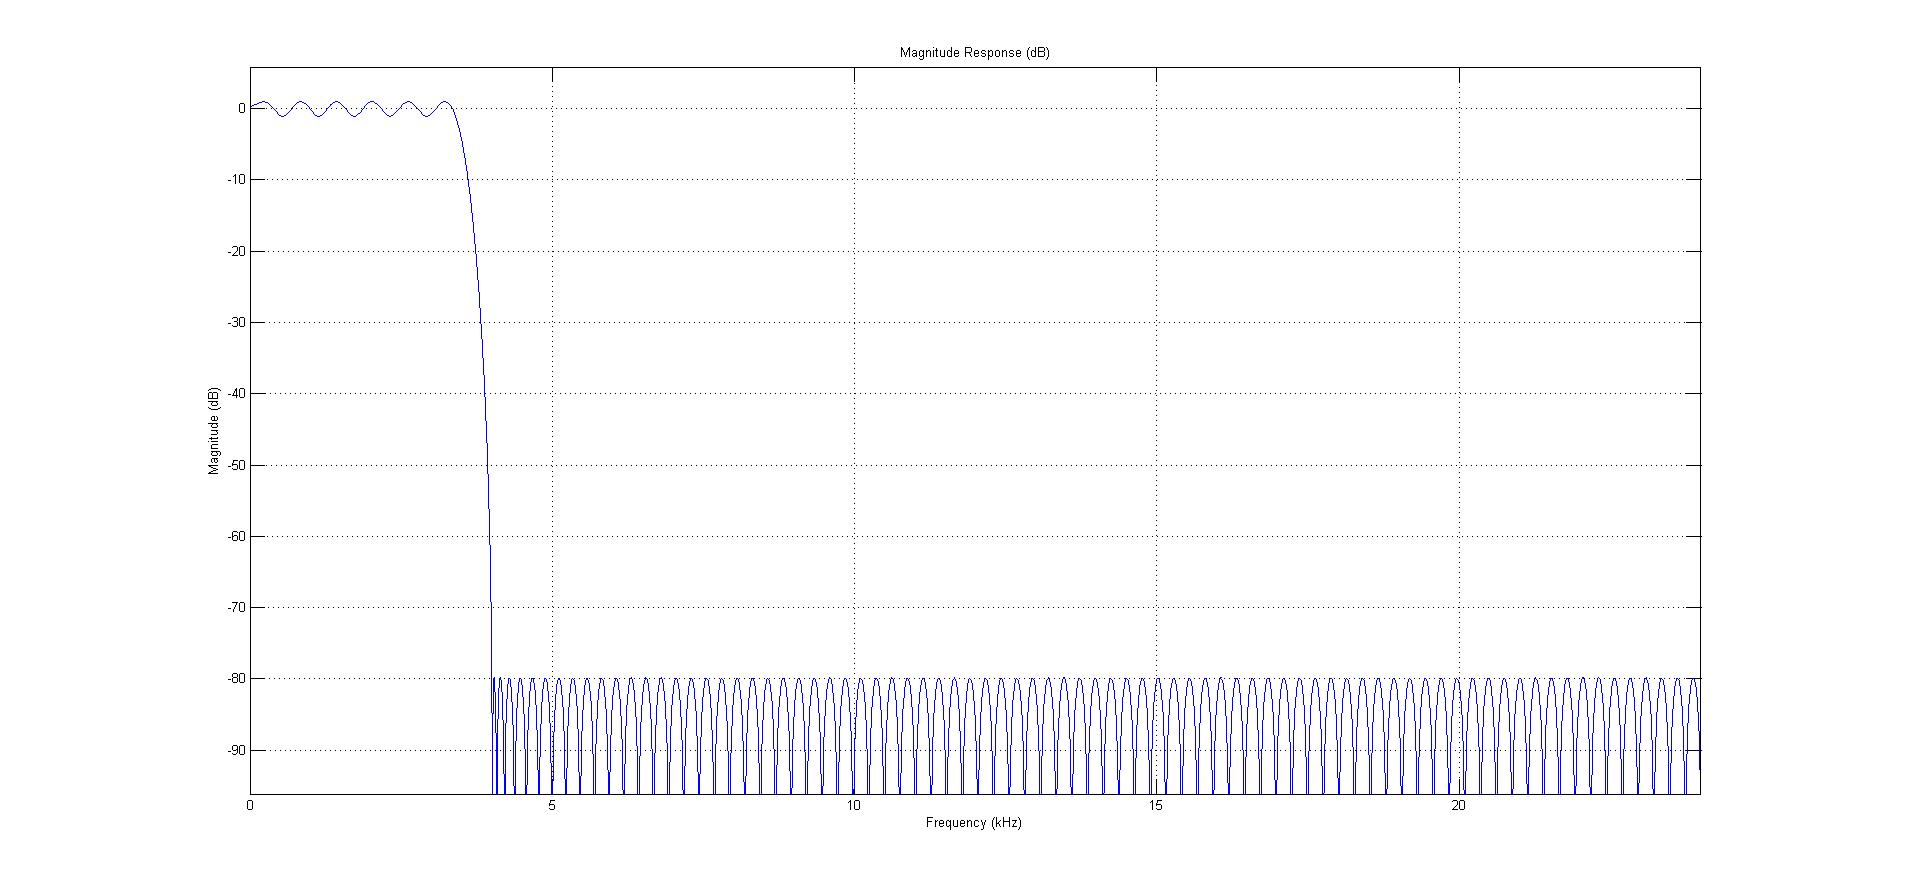
\includegraphics[width=\textwidth]{matlamplitudengang.jpg}
  \caption{Idealer Amplitudengang des erzeugten Filters}
  \label{fig:MatlabAmpgang}
\end{figure}
Im Vergleich dazu soll nun in Abbildung \ref{fig:DSPAmpgang} der reale Amplitudengang gezeigt werden.
\begin{figure}[H]
  \centering
    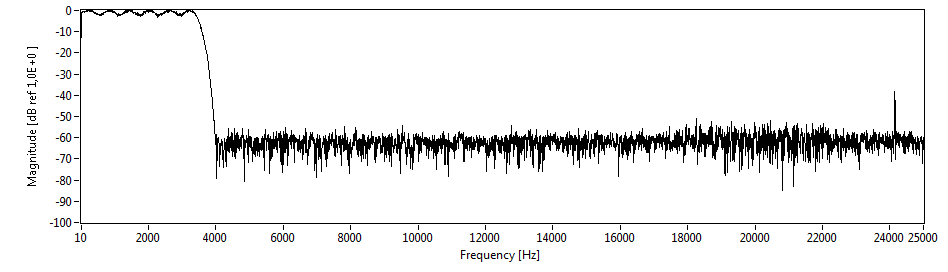
\includegraphics[width=\textwidth]{sqamplitudengang.png}
  \caption{Realer Amplitudengang des erzeugten Filters}
  \label{fig:DSPAmpgang}
\end{figure}
Beide Amplitudeng\"ange \"ahneln einander. Im Durchlassbereich ist im realen Amplitudengang eine leichte D\"ampfung zu erkennen. 
Diese liegt zwischen 1 dB und 2 dB und ist auf die Skalierung von ADC und DAC zur\"uckzuf\"uhren.
Die Grenzfrequenz betr\"agt in beiden Abbildungen ca. 4 kHz.\\
Im Sperrbereich ist deutlich zu erkennen das die D\"ampfung des idealen Amplitudengangs nicht erreicht wird. Es werden lediglich -60 dB erreicht, im idealen Amplitudengang sind es jedoch -80 
dB.\\\par

Die Sprungantwort des idealen Filters ist in Abbildung \ref{fig:MatlabSprung} und die Sprungantwort des realen Filters in Abbildung \ref{fig:DSPSprung} zu sehen.
\begin{figure}[H]
  \centering
    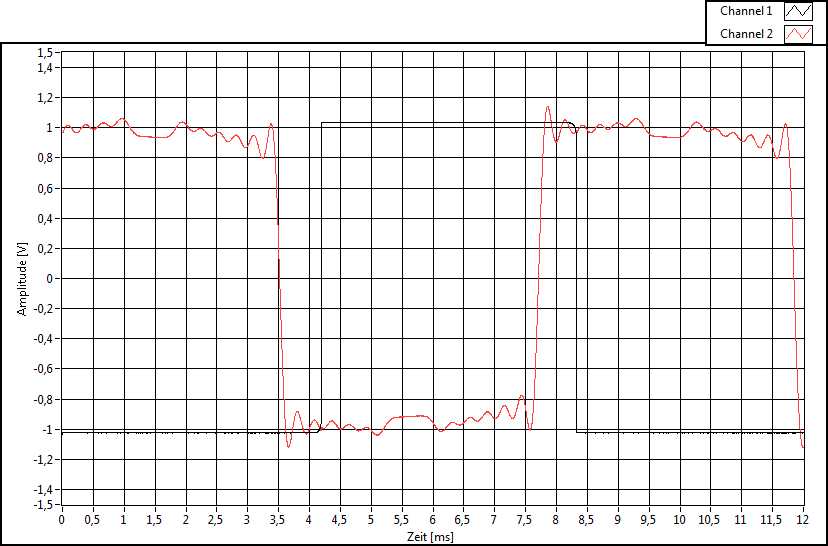
\includegraphics[width=\textwidth]{sq1201vfircomp.png}
  \caption{Reale Sprungantwort des erzeugten Filters}
  \label{fig:DSPSprung}
\end{figure}
\begin{figure}[H]
  \centering
    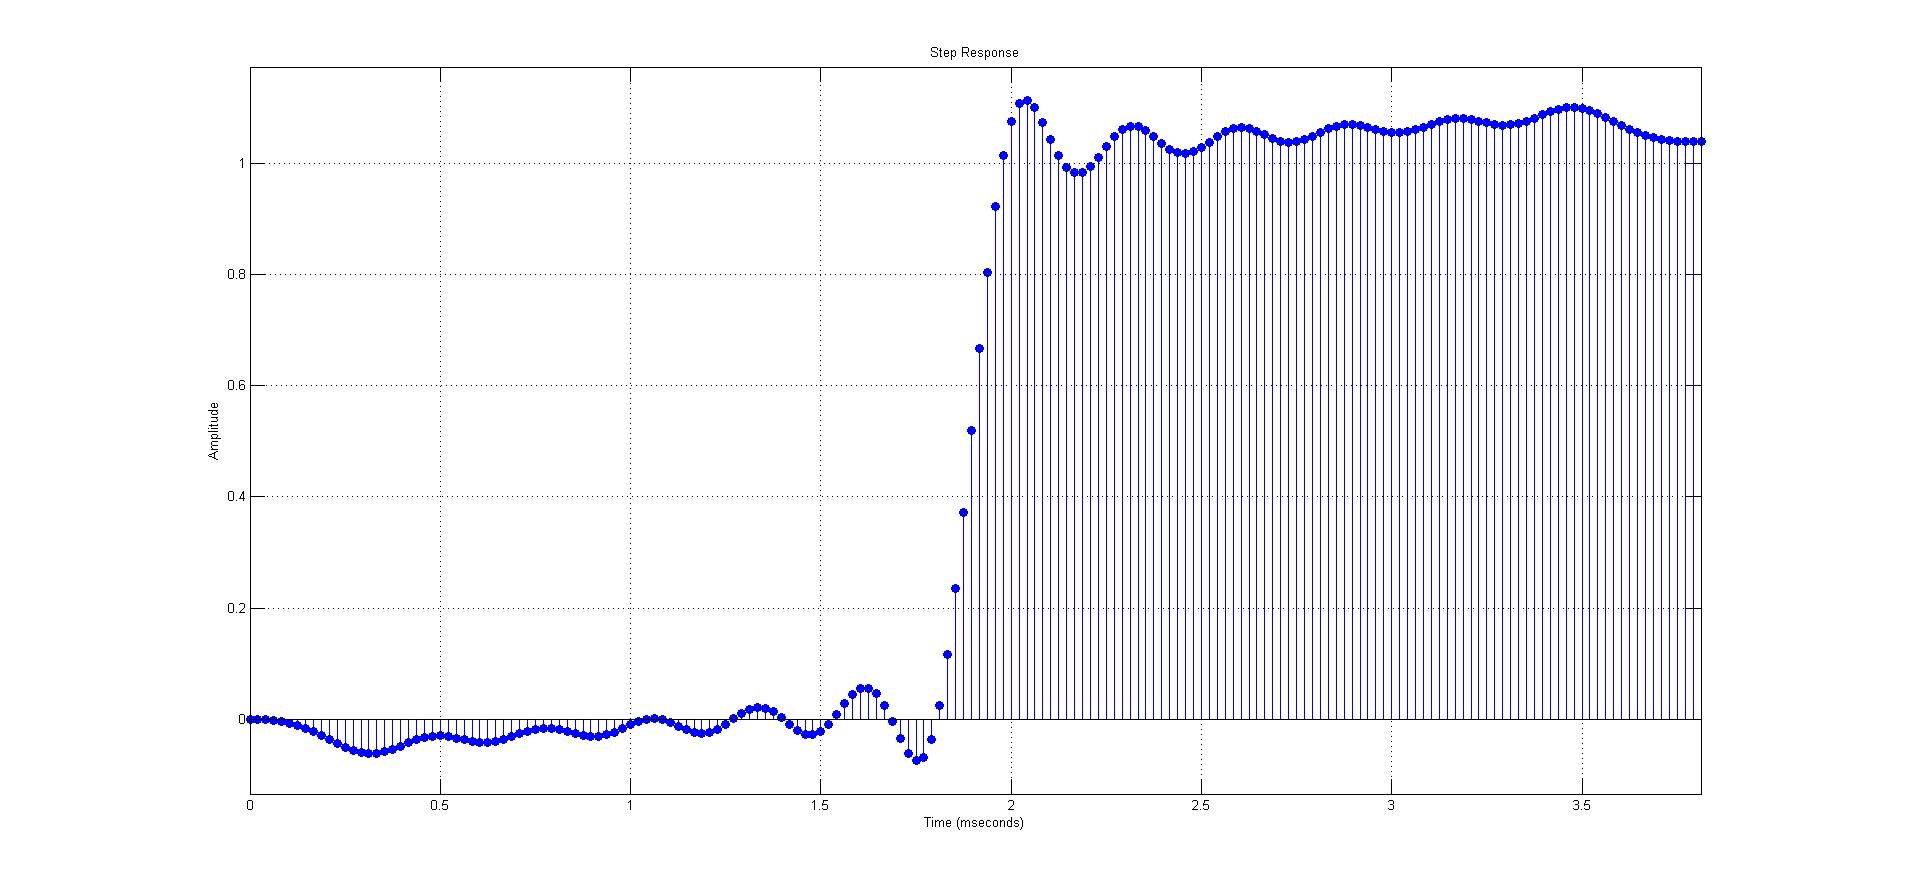
\includegraphics[width=\textwidth]{matlabsprungantwort.jpg}
  \caption{Ideale Sprungantwort des erzeugten Filters}
  \label{fig:MatlabSprung}
\end{figure}
Das Verhalten des realen Filters entspricht sehr genau unseren Erwartungen. Es ist lediglich eine leichte D\"ampfung zu erkennen.
Die Anstiegszeit, sowie das Überschwingverhalten sind fast identisch.

%%Anhang
\begin{appendix}
  \chapter{Quelltext-Dateien}




\end{appendix}

\clearpage\newpage
\listoffigures

\printnoidxglossary[type=\acronymtype,title=Abkürzungsverzeichnis]

\end{document}